% !TEX TS-program = XeLaTeX
% use the following command:
% all document files must be coded in UTF-8
\documentclass[english]{textolivre}
% build HTML with: make4ht -e build.lua -c textolivre.cfg -x -u article "fn-in,svg,pic-align"

\journalname{Texto Livre}
\thevolume{19}
%\thenumber{1} % old template
\theyear{2026}
\receiveddate{\DTMdisplaydate{2026}{2}{13}{-1}} % YYYY MM DD
\accepteddate{\DTMdisplaydate{2026}{4}{23}{-1}}
\publisheddate{\DTMdisplaydate{2026}{9}{25}{-1}}
\corrauthor{Maribel dos Santos Miranda-Pinto}
\articledoi{10.1590/1983-3652.2026.64407}
%\articleid{NNNN} % if the article ID is not the last 5 numbers of its DOI, provide it using \articleid{} commmand 
% list of available sesscions in the journal: articles, dossier, reports, essays, reviews, interviews, editorial
\articlesessionname{articles}
\runningauthor{Miranda-Pinto, Ibáñez-Cubillas and López-Rodríguez} 
%\editorname{Leonardo Araújo} % old template
\sectioneditorname{Daniervelin Pereira~\orcid{0000-0003-1861-3609}}
\layouteditorname{Leonardo Araujo~\orcid{0000-0003-3884-2177}}

\title{Online course for the development of Computational Thinking through ScratchJr using the ADDIE Model}
\othertitle{Curso online para o desenvolvimento do Pensamento Computacional através do ScratchJr utilizando o modelo ADDIE}
% if there is a third language title, add here:
%\othertitle{Artikelvorlage zur Einreichung beim Texto Livre Journal}

\author[1]{Maribel dos Santos Miranda-Pinto~\orcid{0000-0003-0813-1497}\thanks{Email: \href{mailto:maribel.miranda@uab.pt}{maribel.miranda@uab.pt}}}
\author[2]{Pilar Ibáñez-Cubillas~\orcid{0000-0001-7117-5746}\thanks{Email: \href{mailto:pcubillas@uma.es}{pcubillas@uma.es}}}
\author[3]{Slava López-Rodríguez~\orcid{0000-0002-9360-3518}\thanks{Email: \href{mailto:slavalr@ugr.es}{slavalr@ugr.es}}}
\affil[1]{Universidade Aberta, Laboratório de Educação a Distância e eLearning (LE@D), Portugal.}
\affil[2]{University of Málaga, Spain.}
\affil[3]{University of Granada, Spain.}

\addbibresource{article.bib}
% use biber instead of bibtex
% $ biber article

% used to create dummy text for the template file
\definecolor{dark-gray}{gray}{0.35} % color used to display dummy texts
\usepackage{lipsum}
\SetLipsumParListSurrounders{\colorlet{oldcolor}{.}\color{dark-gray}}{\color{oldcolor}}

% used here only to provide the XeLaTeX and BibTeX logos
\usepackage{hologo}

% if you use multirows in a table, include the multirow package
\usepackage{multirow}

% provides sidewaysfigure environment
\usepackage{rotating}

% CUSTOM EPIGRAPH - BEGIN 
%%% https://tex.stackexchange.com/questions/193178/specific-epigraph-style
\usepackage{epigraph}
\renewcommand\textflush{flushright}
\makeatletter
\newlength\epitextskip
\pretocmd{\@epitext}{\em}{}{}
\apptocmd{\@epitext}{\em}{}{}
\patchcmd{\epigraph}{\@epitext{#1}\\}{\@epitext{#1}\\[\epitextskip]}{}{}
\makeatother
\setlength\epigraphrule{0pt}
\setlength\epitextskip{0.5ex}
\setlength\epigraphwidth{.7\textwidth}
% CUSTOM EPIGRAPH - END

% to use IPA symbols in unicode add
%\usepackage{fontspec}
%\newfontfamily\ipafont{CMU Serif}
%\newcommand{\ipa}[1]{{\ipafont #1}}
% and in the text you may use the \ipa{...} command passing the symbols in unicode

% LANGUAGE - BEGIN
% ARABIC
% for languages that use special fonts, you must provide the typeface that will be used
% \setotherlanguage{arabic}
% \newfontfamily\arabicfont[Script=Arabic]{Amiri}
% \newfontfamily\arabicfontsf[Script=Arabic]{Amiri}
% \newfontfamily\arabicfonttt[Script=Arabic]{Amiri}
%
% in the article, to add arabic text use: \textlang{arabic}{ ... }
%
% RUSSIAN
% for russian text we also need to define fonts with support for Cyrillic script
% \usepackage{fontspec}
% \setotherlanguage{russian}
% \newfontfamily\cyrillicfont{Times New Roman}
% \newfontfamily\cyrillicfontsf{Times New Roman}[Script=Cyrillic]
% \newfontfamily\cyrillicfonttt{Times New Roman}[Script=Cyrillic]
%
% in the text use \begin{russian} ... \end{russian}
% LANGUAGE - END

% EMOJIS - BEGIN
% to use emoticons in your manuscript
% https://stackoverflow.com/questions/190145/how-to-insert-emoticons-in-latex/57076064
% using font Symbola, which has full support
% the font may be downloaded at:
% https://dn-works.com/ufas/
% add to preamble:
% \newfontfamily\Symbola{Symbola}
% in the text use:
% {\Symbola }
% EMOJIS - END

% LABEL REFERENCE TO DESCRIPTIVE LIST - BEGIN
% reference itens in a descriptive list using their labels instead of numbers
% insert the code below in the preambule:
%\makeatletter
%\let\orgdescriptionlabel\descriptionlabel
%\renewcommand*{\descriptionlabel}[1]{%
%  \let\orglabel\label
%  \let\label\@gobble
%  \phantomsection
%  \edef\@currentlabel{#1\unskip}%
%  \let\label\orglabel
%  \orgdescriptionlabel{#1}%
%}
%\makeatother
%
% in your document, use as illustraded here:
%\begin{description}
%  \item[first\label{itm1}] this is only an example;
%  % ...  add more items
%\end{description}
% LABEL REFERENCE TO DESCRIPTIVE LIST - END


% add line numbers for submission
%\usepackage{lineno}
%\linenumbers

\begin{document}
\maketitle

\begin{polyabstract}
\begin{abstract}
Computational Thinking (CT) is a pivotal 21st-century competency, increasingly integrated into educational curricula through programming and robotics. However, many teachers lack the interdisciplinary training necessary to incorporate CT across various subjects, highlighting a critical need for professional development programs. This article details the design and evaluation of an online course for educators focused on CT and programming via ScratchJr, utilizing the ADDIE instructional model. Structured into five two-hour autonomous modules, the course offers a flexible learning framework. A qualitative case study was conducted during the implementation and evaluation phases, using questionnaires with undergraduate Pedagogy students. Results indicated a significant enhancement in participants' programming and CT skills, alongside a more favorable outlook toward applying these tools in their future practice. Notably, 96.4\% and 100\% of students positively assessed the integration of these competencies, demonstrating the course's potential to bridge the digital divide in initial teacher training. This initiative was selected for the Scratch Education Collaborative (2022-2024 cohort) and integrated into a MOOC for a Portuguese R\&D project, underscoring its relevance in digital literacy.

\keywords{Computational thinking \sep Programming \sep E-Learning \sep Instructional design \sep Virtual Learning Environments}
\end{abstract}

\begin{portuguese}
\begin{abstract}
O Pensamento Computacional (PC) é uma competência fundamental do século XXI, cada vez mais integrada ao currículo educativo por meio de atividades de programação e robótica. No entanto, muitos professores carecem de formação interdisciplinar em PC que lhes permita incorporá-la em várias disciplinas, o que ressalta a necessidade de programas de educação continuada. Este artigo apresenta a concepção e avaliação de um curso online para o desenvolvimento profissional de educadores em PC e programação usando o ScratchJr, empregando o modelo instrucional ADDIE. O curso está estruturado em cinco módulos de duas horas cada, permitindo uma aprendizagem autónoma e flexível. Foi adotada uma abordagem qualitativa por meio de um estudo de caso durante a fase de implementação e avaliação, aplicando questionários a alunos do curso de Pedagogia. Os resultados da implementação inicial revelaram um aumento significativo nos conhecimentos e habilidades dos participantes em programação e informática, bem como uma percepção mais favorável em relação à sua aplicação na futura prática profissional. 96,4\% e 100\% dos alunos avaliaram positivamente a integração destas competências, evidenciando o potencial do curso para reduzir a exclusão digital na formação inicial. Este curso foi selecionado pela Scratch Education Collaborative para a coorte 2022-2024 e ligado a um MOOC de um projeto português de I\&D, consolidando a sua relevância na formação inicial em competências digitais.

\keywords{Pensamento computacional \sep Programação \sep E-Learning \sep Design instrucional \sep Ambientes Virtuais de Aprendizagem}
\end{abstract}
\end{portuguese}
% if there is another abstract, insert it here using the same scheme
\end{polyabstract}

\section{Introduction}\label{sec-intro}
In recent decades, Computational Thinking (CT) has emerged as a fundamental skill for 21st-century citizens, evolving alongside advances in programming and robotics and their progressive integration into educational curricula. Since \posscite{papert1985logo} seminal proposals, CT has been recognized not only for enhancing higher-order cognitive skills but also for enabling children to explore and reflect upon their own cognitive processes. As \textcite{papert1985logo} noted, by teaching a computer to “think,” children engage in an introspective exploration that transforms them into “epistemologists,” fostering a level of metacognition seldom seen even in adults. This framework was later expanded by \textcite{wing2006computational,wing2008computational}, who posited that CT is not confined to computer science but is a transversal skill as essential as literacy or numeracy. Consequently, contemporary literature underscores the necessity of introducing these competencies during the earliest stages of schooling, seamlessly integrated into daily classroom practices.

Among the tools developed for this purpose, Scratch and ScratchJr are prominent as visual programming languages designed to democratize early access to coding. These platforms foster analytical skills, creativity, collaboration, and problem-solving while promoting playful, multisensory, and meaningful learning experiences \cite{resnick2013designing}. Specifically, ScratchJr—tailored for early childhood education—empowers young learners to construct interactive narratives and games using block-based sequences, which fosters structured narrative and logical reasoning \cite{bers2018scratchjr}.

Specialized literature has demonstrated that early engagement with programming and robotics promotes the development of vital cognitive and socio-emotional competencies. Such experiences allow children to explore novel ways of representing the world, improving spatial orientation, motor coordination, and observational skills \cite{bers2017coding}. Furthermore, through experimentation and structured play, children learn to collaborate, communicate complex ideas, and reflect on their actions, establishing a robust foundation for early digital literacy.

Authors such as \textcite{resnick2013designing,bers2014computational} emphasize the role of play as a catalyst for learning, as it facilitates experimentation, creativity, and problem-solving within meaningful contexts. In this regard, programming serves not merely as a tool for technical acquisition but as a vehicle for fostering social and emotional learning through a constructivist lens.

Aligned with this approach, \textcite{brennan2012new} propose a three-dimensional framework for Computational Thinking (CT). This includes computational concepts (e.g., iteration, parallelism), computational practices (e.g., debugging, remixing), and computational perspectives (the evolving self-perception and worldviews of the designers). This holistic vision underscores the urgency of teacher education programs that enable the coherent and contextualized implementation of these dimensions in the classroom.

However, despite the burgeoning scientific literature and institutional recognition of CT, educational initiatives that systematically integrate it into early childhood and primary education remain scarce.Thus, existing research often focuses on isolated interventions, leaving a gap in evidence regarding sustainable training programs that empower teachers to utilize these tools independently.

Addressing this gap, teacher education—both initial and continuing—assumes a strategic imperative. Distance learning environments offer significant opportunities to equip pre-service and in-service teachers with tools like ScratchJr, fostering pedagogical appropriation and practical application. In this context, the ADDIE instructional model (Analysis, Design, Development, Implementation, and Evaluation) emerges as an effective methodology for designing structured, scalable training tailored to educators' needs.

Consequently, this research aims to design, implement, and evaluate an online course based on the ADDIE model, specifically geared toward CT proficiency and programming with ScratchJr. Developed on the Moodle platform, the course has been implemented in postgraduate contexts and selected by the Scratch Education Collaborative (SEC) for the 2022-2024 cohort. Furthermore, its integration into a MOOC within a Portuguese R\&D project reinforces its international relevance. Thereby, this study seeks to advance professional development by offering an innovative, research-based pedagogical approach that promotes inclusive, creative, and collaborative learning in early education.

\subsection{Literature Review}\label{sec-normas}

\subsubsection{Programming Language for Early Childhood Education}
The introduction of programming languages in early childhood education represents a burgeoning trend in pedagogical innovation, fostering the early development of core cognitive competencies such as Computational Thinking (CT) and problem-solving. These transversal skills facilitate an active and creative engagement with technology from a formative age.

Programming a computer necessitates decomposing complex tasks into sequential steps, formulating precise instructions, and anticipating outcomes—actions that trigger logical reasoning, strategic planning, and metacognition \cite{espadeiro2021pensamento}. Within this framework, children do not merely acquire new modes of expression; they pivot from being passive consumers of information to becoming proactive producers of digital content. This pedagogical shift underpins the design of visual programming tools like ScratchJr and Scratch, which provide accessible, playful, and meaningful environments that stimulate logical reasoning, collaboration, and self-expression \cite{roque2014family,roque2022facilitators}.

From constructivist and sociocultural perspectives, early programming education is anchored in active methodologies that integrate play and experimentation. \textcite[p. 165]{resnick2013designing} emphasize the significance of tinkering and bricolage—learning styles defined by exploration, iteration, and discovery. As they posit, “play is a way of relating to the world, testing limits, and experimenting with new possibilities”. This reinforces the premise that profound learning occurs when students interact with materials and contexts that empower them to externalize and iterate upon their own ideas.

Empirical evidence underscores the positive impact of programming on both cognitive development and socio-emotional maturation. Such findings have catalyzed the adoption of innovative pedagogical frameworks in formal learning environments. In this vein, \textcite{papert1985logo} asserted that CT can be introduced even at the preschool level through programming, enabling children to reflect on their own cognitive mechanisms and develop an epistemological awareness of their learning. This metacognitive dimension is vital for fostering autonomy and learner agency.

Similarly, the Positive Technological Development (PTD) model proposed by \textcite[p. 6]{bers2007positive} provides an integrative framework that bridges technology use with holistic child development. According to this approach, embedding programming into early childhood education can cultivate essential psychosocial assets known as the “5 Cs”: competence, connection, character, confidence, and caring. These dimensions flourish within a healthy and positive educational ecosystem, where children do not merely acquire technical proficiency but also learn to engage in collaboration, explore personal interests, and engage in creative problem-solving. In a similar vein, \textcite{bers2008blocks} argues that the strategic use of mobile devices, such as smartphones and tablets, require a reimagining of pedagogical approaches at this stage, facilitating the creation of engaging and rewarding learning experiences for young children \cite{bers2014computational}.

\subsubsection{Programming ScratchJr}\label{sec-conduta}
ScratchJr is a visual programming language specifically engineered for children aged five to seven, aimed at introducing the fundamentals of Computational Thinking (CT) and digital creation during early childhood \cite{bers2016official}. The platform emerged from an interdisciplinary collaboration between the Developmental Technologies Research Group (DevTech) at Tufts University, the Lifelong Kindergarten group at the MIT Media Lab, and the Playful Invention Company \cite{bers2016official}. Conceived as an adaptation of the original Scratch environment, ScratchJr was tailored to align with the cognitive and psychomotor developmental stages of preschoolers and early elementary students.

Available as a free application for iOS and Android, ScratchJr enables children to construct interactive narratives and animations through a system of graphical blocks representing programmable instructions. Its intuitive interface fosters a hands-on learning environment where pre-literate children can engage with programming, making it uniquely suited for early childhood education.

From a pedagogical standpoint, ScratchJr facilitates more than the acquisition of basic coding concepts, such as algorithms and sequencing; it also cultivates critical thinking and problem-solving prowess. As \textcite[p. 2]{bers2016official} emphasize, “ScratchJr encourages creativity and expression, allowing children to create their own interactive projects through coding”. By designing and manipulating block sequences, children learn to decompose problems into sequential steps and build logical frameworks. This process simultaneously reinforces fine motor skills and hand-eye coordination while enhancing socio-emotional competencies, including collaboration and teamwork \cite{bers2008blocks}.

Furthermore, programming activities with ScratchJr contribute to both socio-emotional and cognitive development by fostering a playful environment that stimulates curiosity and self-directed learning. Consequently, the use of ScratchJr not only facilitates computational literacy but also empowers children to interpret and reflect upon the world around them in an accessible and engaging manner \cite{mirandapinto2020scratchjr}.

Drawing on \posscite[p. 140]{bers2022beyond} "Playground" metaphor, ScratchJr provides open coding spaces where, as she states, “Playgrounds invite fantasy play, imagination and creativity, social interaction, and teamwork; they are spaces to experiment with conflict resolution, and they require less adult supervision”. Within this framework—which aligns with the ideal conditions for learning to code—\textcite{bers2022beyond} further posits that:

\begin{quote}
    In the coding playground, the child is the artist who learns to code, and the paintbrush is the programming language that supports creativity. The colors are the values the child learns and expresses while coding. The coding playground becomes an art studio for practicing a palette of virtues. Creative programming can be a pathway for character development \cite[p. 145-146]{bers2022beyond}.
\end{quote}


Values such as generosity, honesty, patience, curiosity, optimism, and perseverance, which comprise this "palette of virtues," can be effectively cultivated within ScratchJr coding environments. (See \Cref{fig1}).

\begin{figure}[htbp]
\centering
\begin{minipage}{.5\textwidth}
 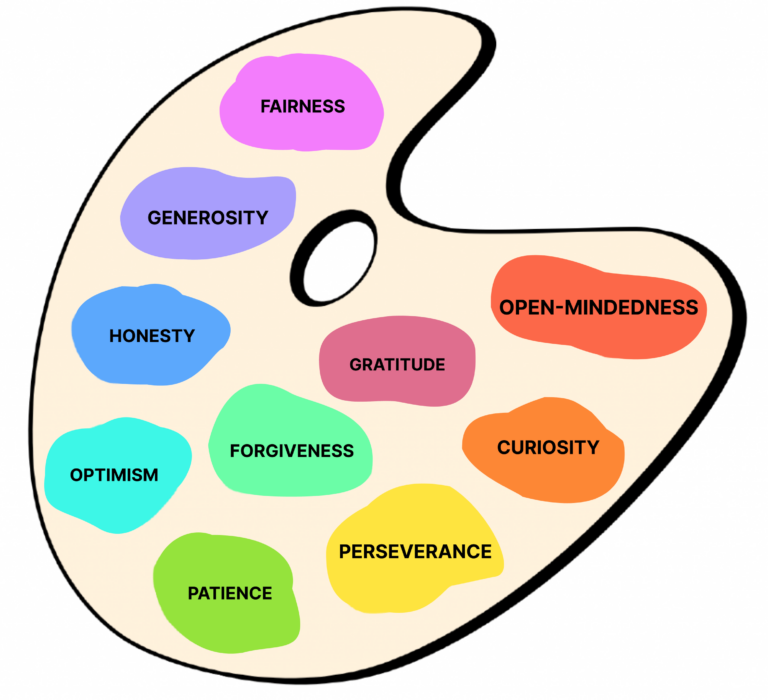
\includegraphics[width=\textwidth]{Fig1.png}
 \caption{The Palette of Virtues.}
 \label{fig1}
 \source{Image retrieved from \textcite[p. 147]{bers2022beyond} and also available in: \url{https://sites.bc.edu/devtech/research-2-2/palette-of-virtues-in-practice}.}
\end{minipage}
\end{figure}

In this regard, the programming environment acts as a catalyst for fostering human values, such as those outlined in \posscite{bers2022beyond} Palette of Virtues. It creates a conducive atmosphere for collaboration and teamwork, enabling children to exchange ideas, engage in collective construction, and reflect on their own creative and cognitive processes when approaching problem-solving.

\subsubsection{Training in Computational Thinking and programming through e-learning for education professionals}\label{sec-fmt-manuscrito}
The development of Computational Thinking (CT) has gained significant traction within the scientific community due to its increasing integration into educational contexts. The conceptual evolution of CT has been shaped by a historical trajectory of researchers committed to redefining how we perceive the acquisition of 21st-century competencies. As argued by \textcite{wing2006computational}, these skills should no longer be viewed as the exclusive domain of computer scientists or engineers but rather as essential literacies for all.

Establishing digital literacy is a prerequisite for advancing toward higher-level programming competencies. Learning to code not only facilitates the mastery of a programming language but also fortifies CT and problem-solving abilities across all disciplines. It is imperative that both educators and students develop foundational digital literacy before engaging in computer programming, which necessitates articulating clear, precise commands to execute tasks through structured sequences. In educational settings, the traditional pillars of literacy and numeracy (reading, writing, and arithmetic) should be integrated with CT activities to enhance children's analytical and reflective capabilities.

Integrating CT and programming into early childhood education demands specialized teacher training, encompassing both initial and continuing professional development. In this regard, tools such as ScratchJr are particularly salient, offering a visual, playful, and meaningful introduction to basic coding. However, for effective classroom implementation, teachers must be equipped not only with technical proficiency but also with the pedagogical strategies necessary for its educational application \cite{bers2018scratchjr,mirandapinto2022scratchjr}.

Pre-service and in-service training in Computational Thinking (CT) and programming empowers educators to acquire essential digital competencies that transcend mere instrumental use, focusing instead on creating innovative, inclusive, and student-centered learning experiences. This professional development is increasingly vital as educators must prepare children to thrive in a pervasively digitalized world, where the ability to solve problems in a logical, structured, and creative manner is paramount.

In this context, distance education via e-learning environments offers an effective and accessible alternative for teacher education. As \textcite{ibanez2018aspectos} notes, e-learning in its various forms generates learning opportunities that allow educators to access specialized knowledge without the logistical constraints of traditional face-to-face formats. By offering flexibility in both time and space, this modality aligns with the professional realities of teachers, facilitating their active and sustained engagement in continuous professional development, as evidenced by the positive outcomes reported by \textcite{amante2019computational,amante2023designing,souza2020evaluation}.

However, for online training to be effective, it must be rooted in robust pedagogical principles. After all, the quality of an e-learning initiative depends on its instructional design—defined as the systematic planning of objectives, content, activities, resources, and assessment. Consequently, it is necessary to ensure constructive alignment between learning objectives, proposed activities, support materials, and assessment criteria \cite{hadi2017development}. Designing online programs under these principles not only guarantees internal consistency and pedagogical relevance but also amplifies their impact on actual classroom practice, a correlation substantiated by the research of \textcite{quintas2022learning,amante2023designing}.


\subsubsection{ADDIE Instructional Model}\label{sec-formato}
Instructional Design (ID), defined as “a systematic method for developing educational and training programs aimed at improving student performance” \cite[p. 149]{hadi2017development}, is a cornerstone in the planning, production, and implementation of training initiatives within virtual environments. ID models provide a structured and systematic framework to organize the processes inherent in creating educational activities, thereby ensuring the quality and efficacy of distance learning \cite{raposo2020innovacion}.

The ADDIE model—an acronym for Analysis, Design, Development, Implementation, and Evaluation—was established in 1975 by the Center for Educational Technology at Florida State University, initially tailored for the U.S. military. However, it was not until 1978, following the work of Dick and Carey, that the model emerged as a benchmark for educational and training program design \cite{hadi2017development}.

Rooted in human knowledge systems theory and the information processing paradigm, the ADDIE model ensures that the outputs of each phase are evaluated before advancing to the next, fostering continuous evaluation and feedback (Maribe, 2009). The interaction between these elements constitutes a five-stage instructional cycle, each with a distinct purpose \cite{maribe2009instructional,spatioti2022comparative}:

\begin{itemize}
    \item  Analysis: Identifying the core needs of the target audience and assessing students' prior knowledge and competencies.
    \item Design: Defining the learning environment and curriculum, including objectives, content, activities, and assessment tools. This phase demands precision and a systematic approach.
    \item Development: Producing instructional materials and integrating technological resources, specifically for online learning environments.
    \item Implementation: Deploying the final product within the intended learning environments, involving continuous adjustments to optimize performance.
    \item Evaluation: Systematically assessing training effectiveness. This includes formative evaluation (process-oriented) and summative evaluation (outcome-oriented).
\end{itemize}

After evaluating alternative models—such as those proposed by Dick and Carey, Gagné, or the ASSURE model—ADDIE was selected for its capacity to facilitate ICT-mediated autonomous learning and its inherent simplicity, which enhances efficiency in course creation (Maribe, 2009). Furthermore, ADDIE is widely utilized to design, develop, and evaluate distance learning experiences and digital educational content \cite{trust2018using,raposo2020innovacion}.

This article details the design and development of an open online course aimed at the pre-service and in-service training of teachers in Computational Thinking (CT) and programming via ScratchJr. The goal is to provide the academic community with a framework for initial and continuing education that promotes meaningful, rigorous, and autonomous learning among educators.


\section{Materials And Methods}\label{sec-modelo}
The objective of this study was to design and develop an open online course on ScratchJr for the pre-service and in-service training of education professionals, utilizing the ADDIE instructional design model. To achieve this, a qualitative approach was adopted through a case study framework. As \textcite[p. 11]{stake2005investigacion} defines it, a case study involves “the study of the particularity and complexity of a single case, in order to understand its activity in important circumstances”. In the context of curriculum development, adhering to the phases of an instructional design model is imperative to ensure that planned activities align with learning objectives and facilitate an effective evaluation of outcomes.

The study sample comprised 48 third-year undergraduate students enrolled in the Bachelor’s Degree in Pedagogy at the University of Malaga, all of whom completed the initial questionnaire and participated in the training. The initial cohort included 81.3\% (n=39) women and 18.8\% (n=9) men, with ages ranging from 20 to 25 years. Upon conclusion of the course, 28 students submitted their final ScratchJr projects and completed the exit questionnaire—both of which were mandatory requirements for course completion and the issuance of a certificate by the @rcaComum Association. Of these 28 participants, 78.57\% (n=22) were women and 21.42\% (n=6) were men, aged between 20 and 24.

\subsection{Analysis}\label{sec-titulo}
During the Analysis phase, the target audience was identified, and comprehensive assessments were conducted to determine the specific training needs of education professionals regarding Computational Thinking (CT) and programming with ScratchJr. This analysis drew upon longitudinal data from the @rcaComum \cite{mirandapinto2009processos} and Kids Media Lab projects, supplemented by a review of existing literature and the application of engagement scales to both pre-service and in-service educators \cite{mirandapinto2019programacion,mirandapinto2019aprender}. These instruments were pivotal in mapping participants' prior knowledge and target competencies, as well as identifying systemic barriers to the integration of programming technologies within educational settings.

\subsubsection{Data collection and initial Data collection and initial analysis}\label{sec-autores}
The @rcaComum project (2005–2009) was an Ibero-American online community for education professionals and researchers, designed to facilitate the exchange of best practices and experiences regarding ICT integration within Early Childhood and Primary Education curricula. During this period, semi-structured interviews and content analysis of community forums \cite{mirandapinto2009processos} were employed to identify key areas of interest and the competencies required for effective technology integration. These data revealed a pronounced demand for training in Computational Thinking (CT) to bolster digital literacy from an early age. While the community achieved significant international reach and representation, its focus was subsequently expanded through the Kids Media Lab project (2016–2018). This successor project integrated these foundational principles into specialized training in CT, programming, educational robotics, and internet safety, directly addressing the needs identified within @rcaComum and the continuous evaluation of its activities \cite{ibanez2018aspectos,mirandapinto2012ambientes,mirandapinto2010colaboracion}.

\subsubsection{Justification of the target audience and training needs}\label{sec-idioma}
Data gathered across these initiatives, particularly within the Kids Media Lab project, underscore the pressing need for professional development in Computational Thinking (CT) using ScratchJr and Scratch. Qualitative analysis of the questionnaires revealed that most early childhood educators lacked foundational programming skills, which constrained their capacity to integrate these concepts into their pedagogical practice. Furthermore, three critical needs were identified: (1) the development of fundamental coding literacy for novice teachers; (2) training on the curricular integration of ScratchJr and Scratch across early childhood and primary education subject areas; and (3) the establishment of a Community of Practice (CoP) to facilitate the exchange of experiences and bolster teachers' self-efficacy in classroom technology use \cite{mirandapinto2017laboratory}.



\subsubsection{Course design and learning objectives}\label{sec-resumo}
Based on these findings, the course was designed as a flexible, autonomous, and self-paced program, tailored for both pre-service and in-service educators. Developed under the Laboratório de Tecnologias e Aprendizagem de Programação (KML II) project, this training was structured in a modular format, spanning from the foundational concepts of Computational Thinking (CT) to the execution of practical application projects using ScratchJr and Scratch. The course objectives were specifically formulated to bridge the identified knowledge gaps, focusing on the acquisition of practical competencies to foster the pedagogical integration of programming in early childhood and primary education \cite{mirandapinto2017laboratory}.

This analysis phase established a robust evidence base that informed the creation of specialized content tailored to teachers' specific requirements. The granular identification of the target audience and their developmental needs enabled the precise calibration of learning objectives, materials, and activities, thereby ensuring constructive alignment with the interests and professional demands of the target group.

\subsection{Design}\label{sec-secoes}
In this phase, the training structure of the ScratchJr learning course is planned, adapting it to the findings of the analysis phase and aligning each component with the identified needs of the target audience. The course is designed as an e-learning program so that teachers and educators, both in initial training and in practice, can access the content in a flexible and self-managed way. This choice responds to the data collected, which indicated time constraints among participants, making it necessary to have a structure that could be adapted to different paces and schedules.

\subsubsection{Course structure and content organization}\label{sec-format-simple}
The course duration was established at five days, with a recommended commitment of two hours per day of asynchronous study, though this remains flexible to accommodate the individual interests and learning paces of the participants. To facilitate the development of Computational Thinking (CT) and programming competencies, the content is structured around several core components: thematic introduction, learning objectives, instructional materials, learning activities, assessment, and supplemental reading. These elements were organized using a planning grid (\Cref{tbl1}), informed by the \textcite{mcgee2012blended} alignment model, to ensure rigorous correspondence between objectives, activities, and assessment criteria.

{
\scriptsize
\setlength{\tabcolsep}{3pt} 
\begin{longtable}{>{\raggedright\arraybackslash}p{1.1cm} >{\raggedright\arraybackslash}p{2cm} >{\raggedright\arraybackslash}p{0.75cm} >{\raggedright\arraybackslash}p{3.3cm} >{\raggedright\arraybackslash}p{3.3cm} >{\raggedright\arraybackslash}p{3cm}}
\caption{ScratchJr course planning.}
\label{tbl1}
\\
\toprule
\multicolumn{6}{c}{COURSE ScratchJr} \\
\midrule
Week & Content & Objec\-tive & Activities & Resources and materials &
Evaluation  \\
\midrule
Day 1 \newline 
(2 hours) &

ScratchJr App

ScratchJr Interface

ScratchJr Paint Editor

ScratchJr Blocks

ScratchJr Community

Coding

Algorithms &

LO 1

LO 2

LO 3

LO 4

LO 8 &

1st hour

See the document Information and install the ScratchJr APP, if possible, on a tablet;

Visit the website \url{https://www.scratchjr.org and watch the ScratchJr}introductory video available at \url{https://www.scratchjr.org/about/info};  

Explore the resources available in the Learn Menu and the Teach Menu on the \url{https://www.scratchjr.org website}.

Sign up to the ScratchJr Connect community \url{http://scratchjr.org/}teach/connect

2nd hour

Read the text "Taking coding home: analysis of ScratchJr usage in home and school settings".

Do the "Algorithms" activity, available in the PDF "Algorithm ScratchJr.pdf". &

Mandatory video:

ScratchJr video presentation (\url{https://www.scratchjr.org/about/info})

Obligatory readings:
\begin{itemize}
    \item Interface guide
    \item Paint Editor Guide
    \item Block Guide
    \item Taking coding home with you: an analysis of the use of ScratchJr in home and school environments.
\end{itemize}
 
Reference materials or activities:
\begin{itemize}
    \item ScratchJr planning Information
    \item ScratchJr Algorithm
\end{itemize}

Optional reading:
\begin{itemize}
    \item Teaching tools, teachers' rules: exploring the impact of teaching styles on young children's programming knowledge in ScratchJr.
\end{itemize}
&

Discussion forum: share ideas, questions and reflections with fellow students on the required reading and solving the algorithms.

Send the resolution of the "Algorithms" activity to the email \href{mailto:geral@kidsmedialab.pt}{geral@kidsmedialab.pt} \\

Day 2 \newline 
(2 hours) &
Coding

ScratchJr App

ScratchJr Interface

ScratchJr Paint Editor

ScratchJr Blocks &

LO 1

LO 2

LO 5

LO 6

LO 7

LO 8 &

1st hour

Carry out the Coding Cards activities (Activity 1 and Activity 2).

2nd hour

Carry out the activity "Coding Cards" (Activity 3).

Start the "Final Project Design with ScratchJr". Make the project design (storyboard) in four 4 pages, in ScratchJr. &

Activity materials:

Coding Cards activity 1

Coding Cards activity 2

Coding Cards activity 3

Designing the final project with ScratchJr

Optional reading:

Designing ScratchJr: support for early childhood learning through computer programming &

Send the resolution of the "Coding Cards" activities to the email \href{mailto:geral@kidsmedialab.pt}{geral@kidsmedialab.pt}

Discussion forum: Share your ideas and questions about the design and creation of your project with your peers. \\
Day 3\newline 
(2 hours) &

ScratchJr App

ScratchJr Interface

ScratchJr Paint Editor

ScratchJr Blocks

Coding

Algorithms &
LO 1

LO 2

LO 7

LO 8 &

1st hour

Continued "Designing the Final Project with ScratchJr".

2nd hour

Start creating the game or story in ScratchJr. Spend this hour on the first page, creating the scenario and programming the different actors. &
Activity materials:

Diseñar el proyecto final con ScratchJr

Optional reading:

Constructing the ScratchJr programming language in the early childhood classroom.

 Discussion forum: Share your ideas and questions about the design and creation of your project with your peers. \\
Day 4\newline 
(2 hours) &

ScratchJr App

ScratchJr Interface

ScratchJr Paint Editor

ScratchJr Blocks

Coding

Algorithms &

LO 1

LO 2

LO 7

LO 8 &

1st hour

Continue with the creation of the game or story in ScratchJr. Spend this hour on the 2nd page, creating the scenario and programming the different actors.

2nd hour

Continue with the creation of the game or story in ScratchJr. Spend this hour on the 3rd page, creating the scenario and programming the different actors. &

Activity materials:

Diseñar el proyecto final con ScratchJr

Optional reading:

Programming with ScratchJr: a review of the first year of user analytics &

 Discussion forum: Share your ideas and questions about the design and creation of your project with your peers. \\
Day 5 \newline 
(2 hours) &

ScratchJr App

ScratchJr Interface

ScratchJr Paint Editor

ScratchJr Blocks

Coding

Algorithms &

LO 1

LO 2

LO 7

LO 8 &

1st hour

Continue with the creation of the game or story in ScratchJr. Spend this hour on the 4th page, creating the scenario and programming the different actors.

2nd hour

At the end, share your ScratchJr project with your classmates on the course platform and by email. &

Activity materials:

Designing the final project with ScratchJr

Optional reading:

Bibliography &

Send the final project to the email: \href{mailto:geral@kidsmedialab.pt}{geral@kidsmedialab.pt}

Discussion forum: Share your final project and comment on the projects of your peers and comment on what you liked. \\
\bottomrule
\source{Author’s own elaboration.}
\end{longtable}
}





\subsubsection{Learning objectives and specific competencies}\label{sec-links}
The Learning Objectives (LOs) were defined to ensure each represents a practical, transferable skill applicable to educators' professional practice. These objectives follow a scaffolded progression, ranging from initial exploration and mastery of the interface (LO1–LO3) to the independent creation and presentation of an original project (LO7). This sequence aims to cultivate an increasing level of proficiency, moving from foundational familiarization to creative application and reflection on pedagogical practice:

\begin{itemize}
    \item LO1: Identify the core features of the ScratchJr application, relating them to programming principles and justifying its suitability for early childhood education.
    \item LO2: Explore the ScratchJr interface to evaluate its affordances and limitations for curricular integration in preschool.
    \item LO3: Analyze ScratchJr activities integrated into the curriculum by examining exemplars from the official website, ScratchJr Connect, and provided resources.
    \item LO4: Register and engage with the ScratchJr Connect community.
    \item LO5: Articulate and describe programmed actions within the ScratchJr environment.
    \item LO6: Execute and adapt Coding Card activities within the platform.
    \item LO7: Design and develop a comprehensive original project in ScratchJr.
    \item LO8: Collaborate with peers to discuss experiences, resolve queries, and share insights regarding programming.
\end{itemize}


\subsubsection{Evaluation and reflection}\label{sec-listas}
To reinforce learning, the course incorporates formative assessment activities where participants receive feedback from both tutors and peers, fostering a culture of reflective and collaborative evaluation. In the final stage, the exchange of experiences is prioritized, so, participants share their capstone projects within the ScratchJr Connect community and engage in dialogue regarding their challenges and achievements. This interaction not only facilitates collective knowledge construction but also fosters the development of a professional Community of Practice (CoP) dedicated to the integration of ScratchJr in early childhood education.



\subsection{Development}\label{sec-figuras-tabelas}
During the Development phase, the ScratchJr course is instantiated on the Moodle learning platform within the @rcaComum community. This stage is primarily operational, as it involves the production, structuring, and organization of instructional materials and the Virtual Learning Environment (VLE). These actions are strictly informed by findings from the analysis and design phases to ensure the pedagogical and functional coherence of the course.


\subsubsection{Production of teaching materials}\label{sec-quotesandfootnotes}
Guided by the learning objectives and the structural blueprint established during the design phase, instructional materials were developed to include readings, guides, tutorials, and interactive ScratchJr exemplars. Each resource was designed to be clear, visually engaging, and practice-oriented, fostering autonomous learning while remaining adaptable to the diverse needs and contexts of the participants. Key resources include:

\begin{itemize}
    \item Theoretical Readings: open-access scientific literature was provided in PDF format to ensure equitable access to core theoretical content.
    \item Step-by-Step Guides: instructional documents with detailed procedural steps were created to empower participants to navigate ScratchJr independently. These guides feature visual aids and annotated screenshots illustrating each phase of tool utilization.
    \item Video Tutorials and Interactive Exemplars: fundamental concepts—such as project creation and the application of Coding Cards—were addressed through video tutorials hosted on the official ScratchJr Connect platform, providing dynamic demonstrations of the software in action.
\end{itemize}


\subsubsection{Design of the virtual learning environment}\label{sec-equacao}
The Moodle platform was configured to provide an intuitive and streamlined environment, facilitating seamless access to instructional materials and enabling participants to progress through the curriculum in a clear, structured manner. The course was organized into thematic modules that align with the predefined learning objectives, designed to guide participants from foundational concepts toward the development of their final projects. Figures \ref{fig2}, \ref{fig21}, \ref{fig3}  illustrate the architectural layout and the technological resources integrated into the ScratchJr course.

\begin{figure}[htbp]
\centering
\begin{minipage}{.5\textwidth}
 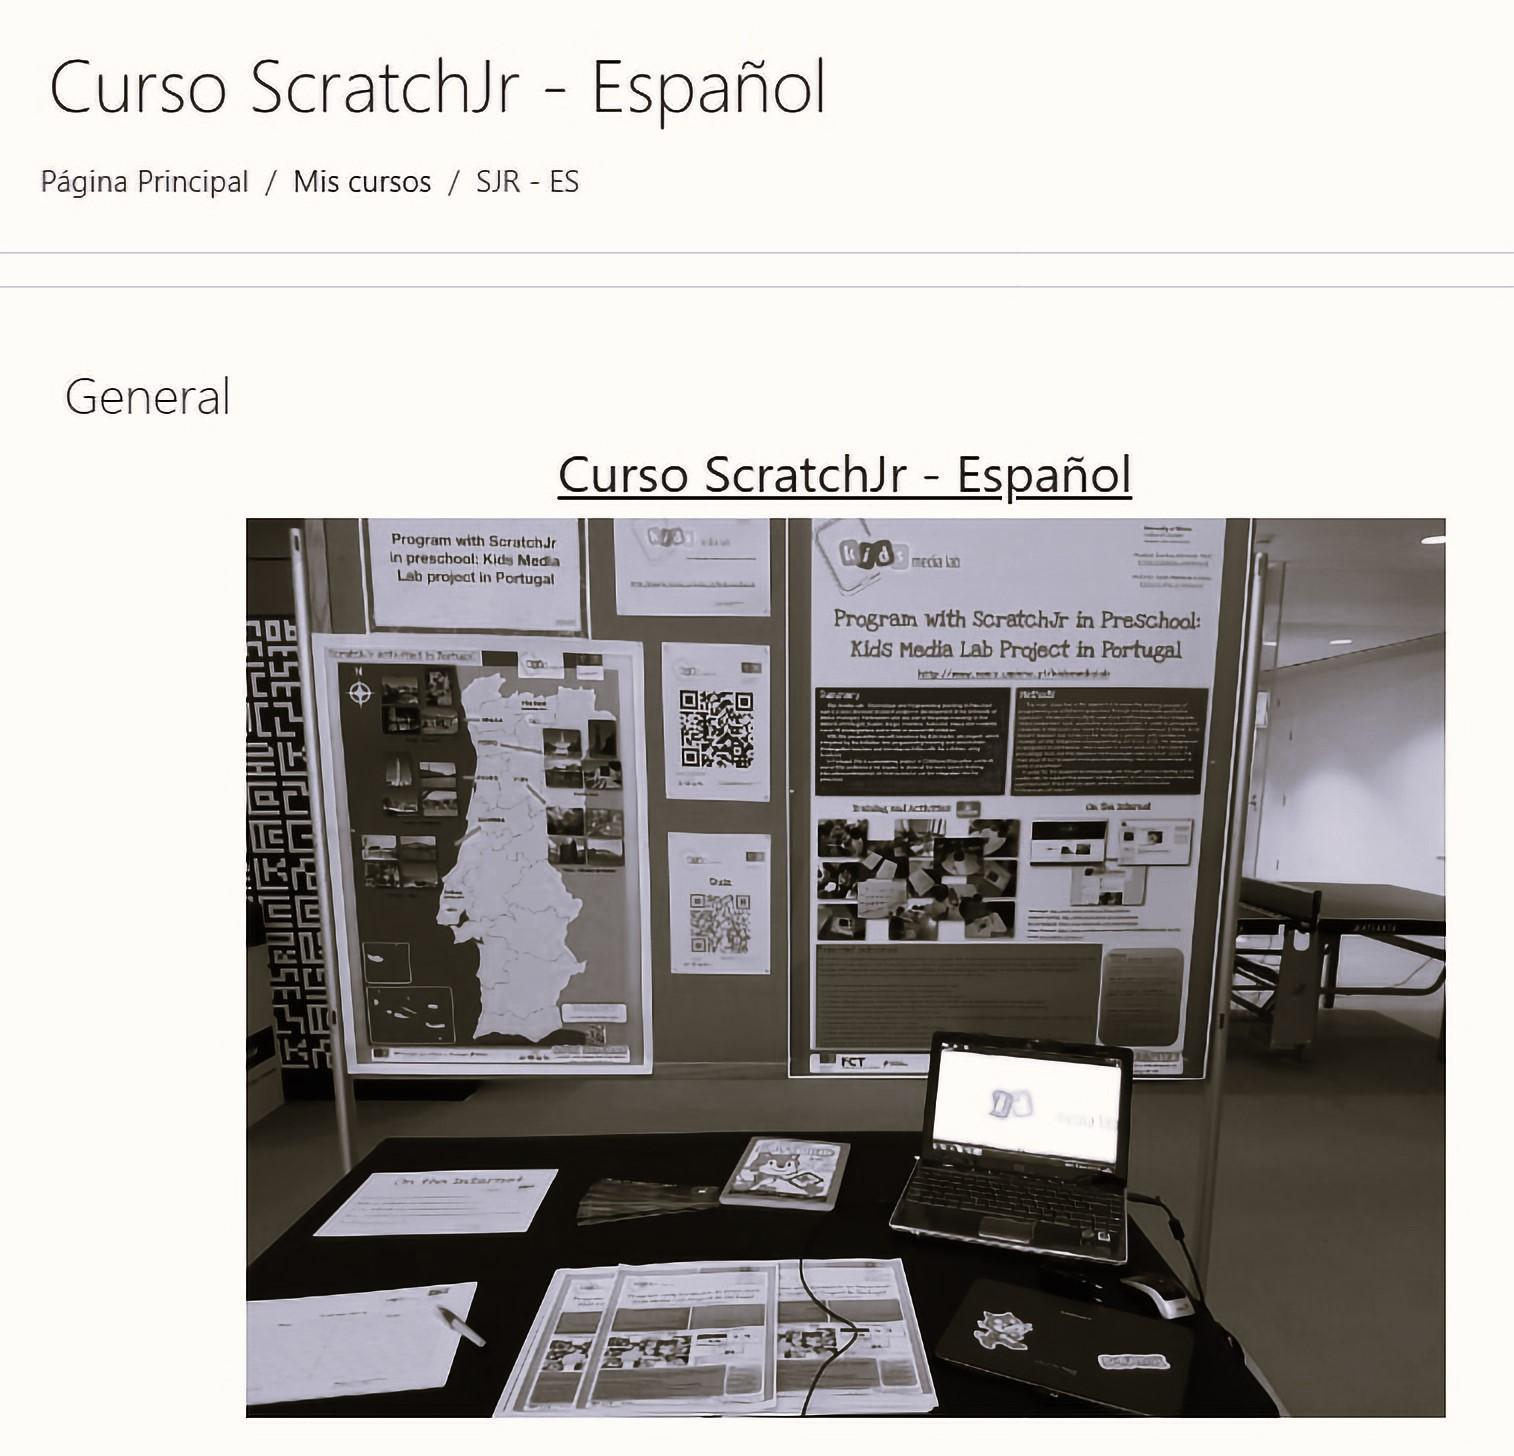
\includegraphics[width=\textwidth]{Fig2.png}
 \caption{Structure of the ScratchJr course—header, first section, and second section—.}
 \label{fig2}
 \source{Author’s own elaboration.}
\end{minipage}
\end{figure}

\begin{figure}[htbp]
 \centering
 \begin{minipage}{.45\textwidth}
 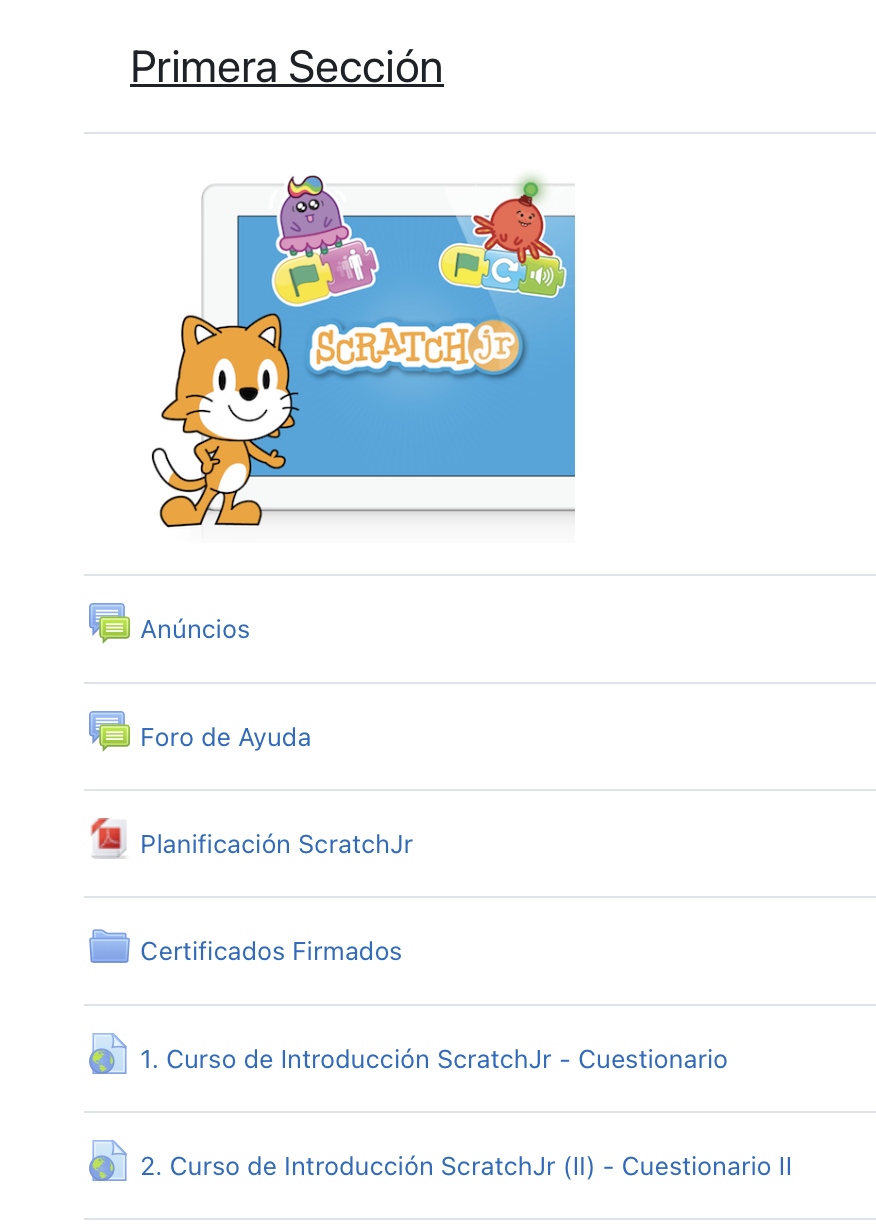
\includegraphics[width=\textwidth]{Fig21.png}
 \end{minipage}%
 \qquad
 \begin{minipage}{0.45\textwidth}
 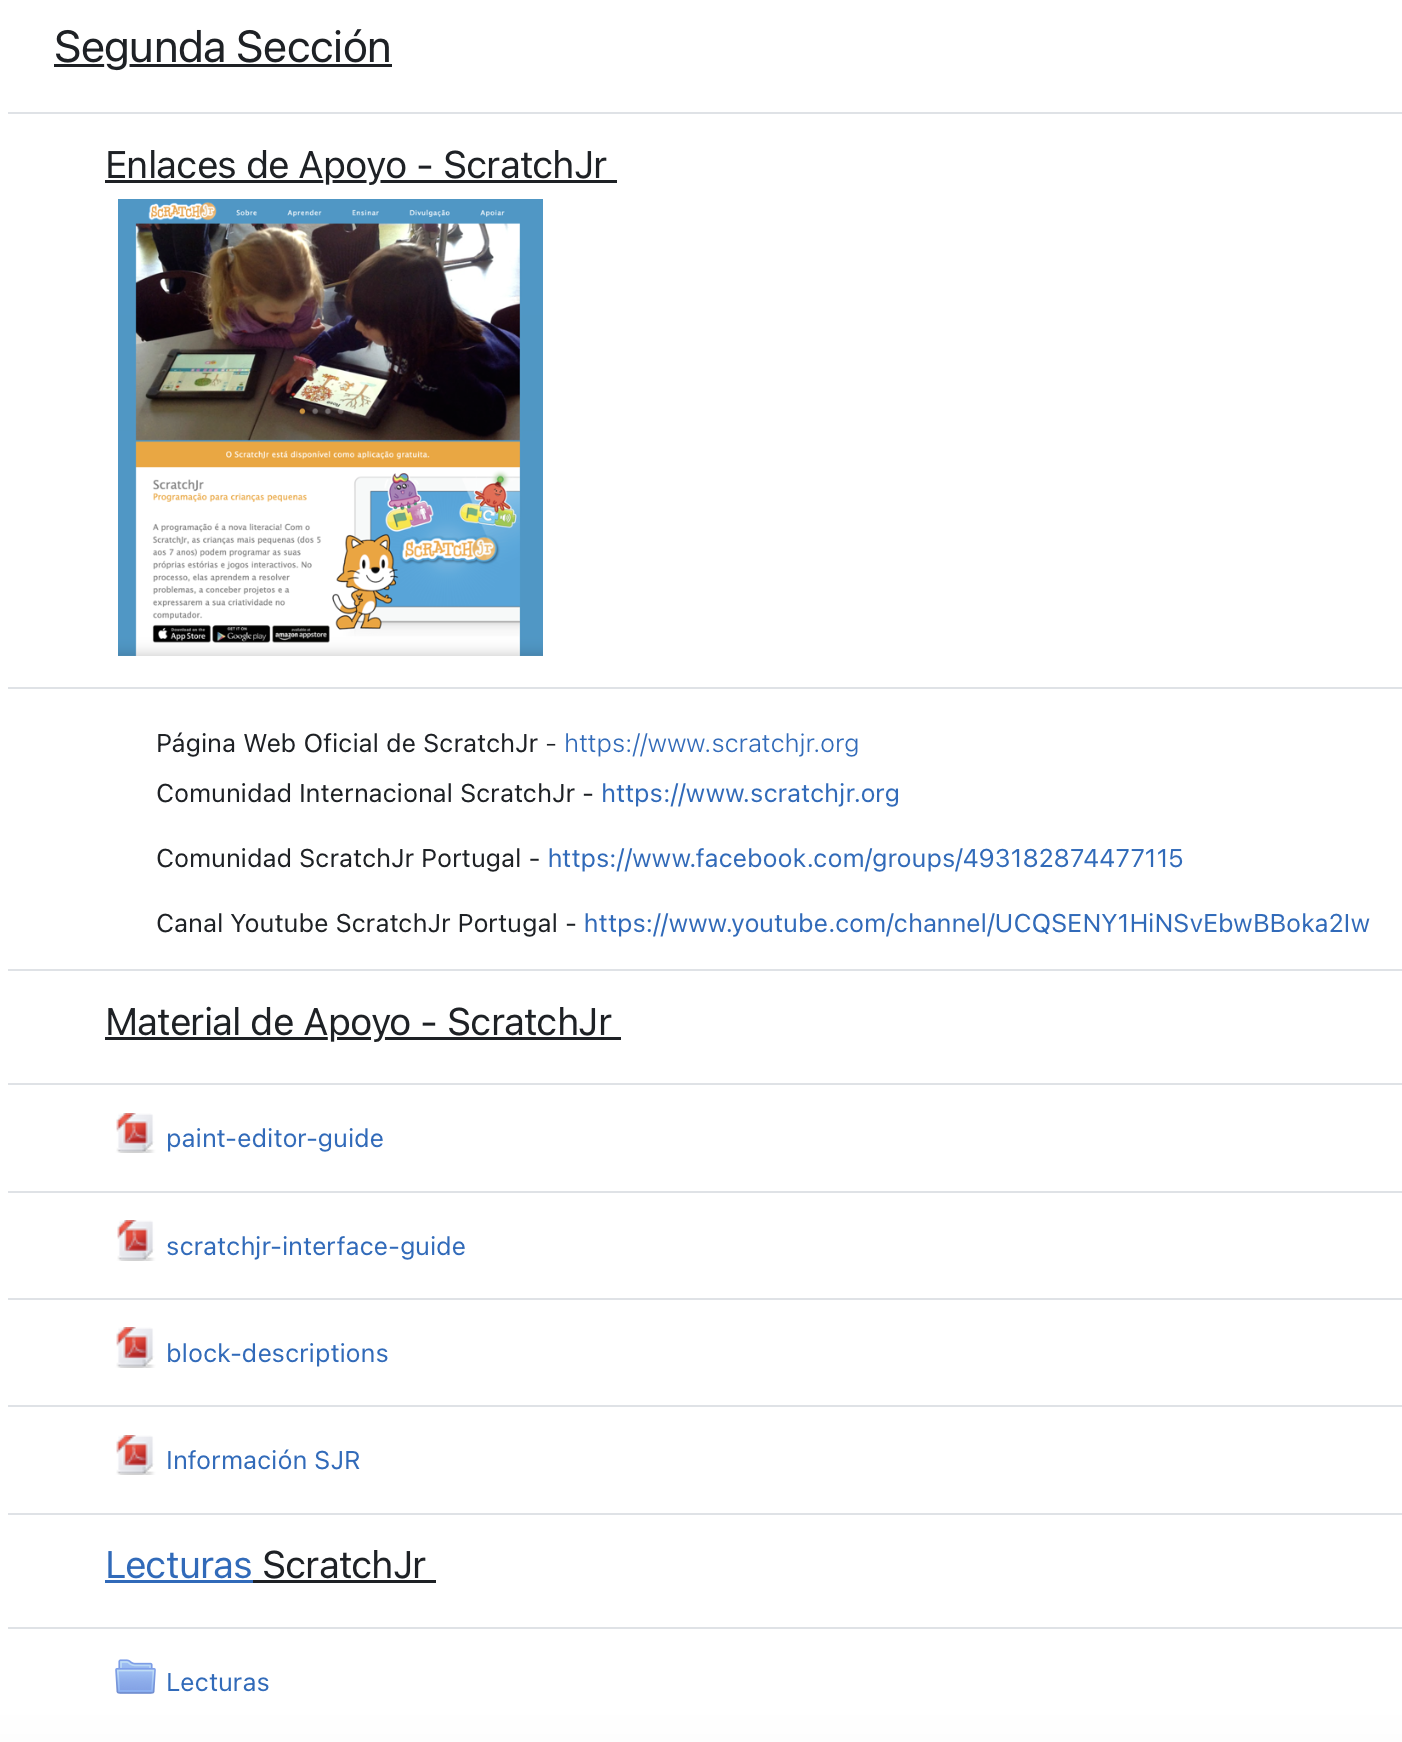
\includegraphics[width=\textwidth]{Fig22.png}
 \end{minipage}%
 \caption{Structure of the ScratchJr course—header, first section, and second section—.}
 \label{fig21}
 \source{Author’s own elaboration.} 
\end{figure}

\begin{figure}[htbp]
 \centering
 \begin{minipage}{.50\textwidth}
 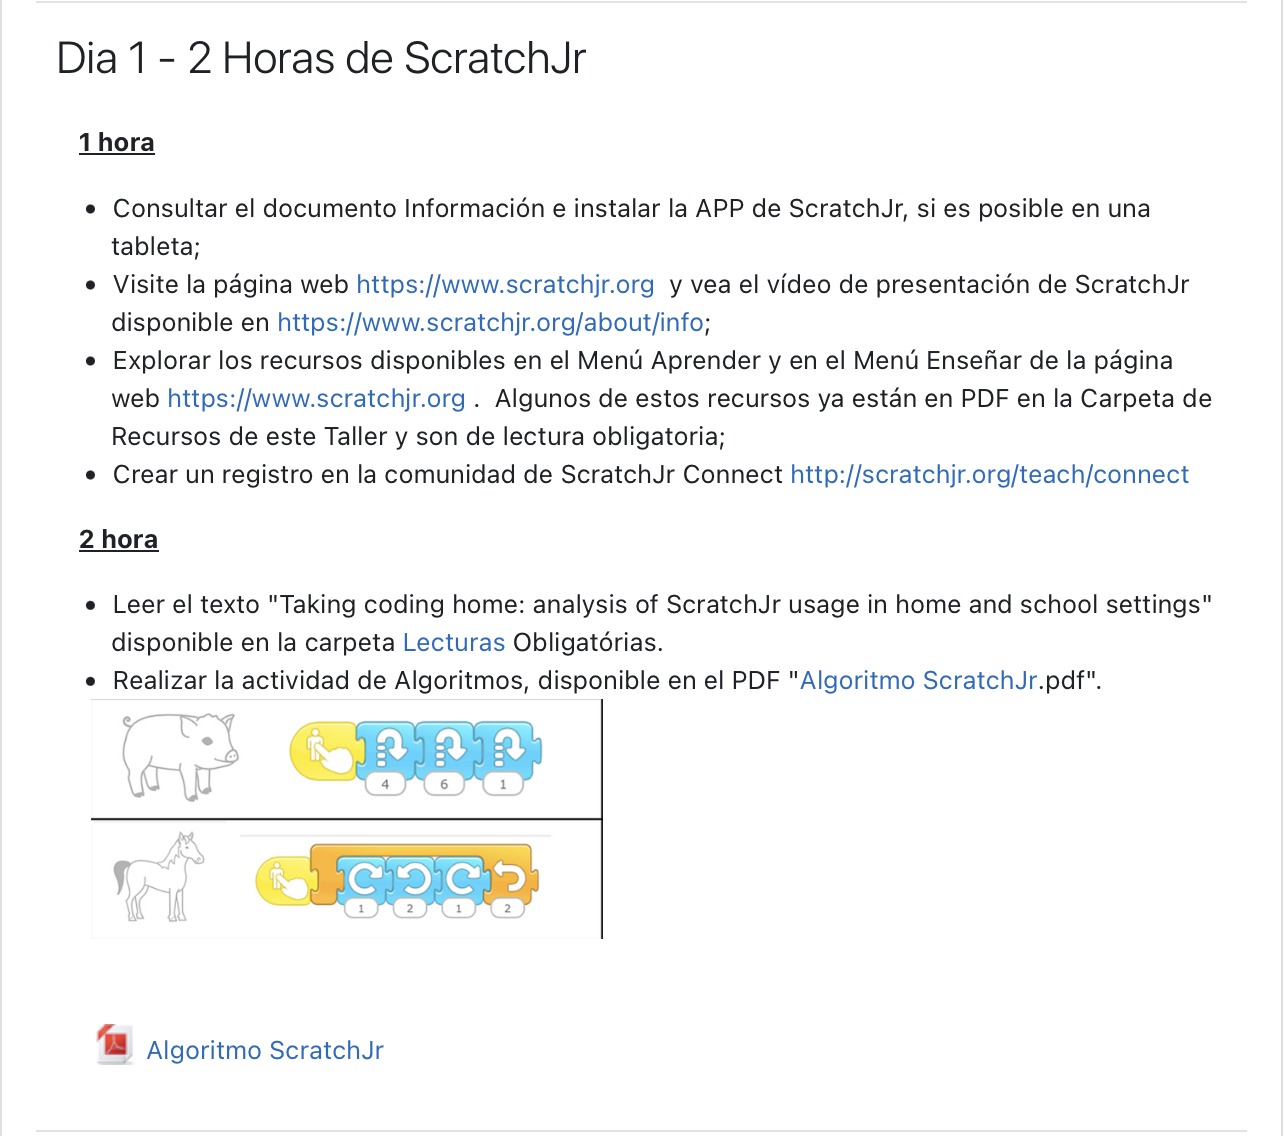
\includegraphics[width=\textwidth]{Fig3.png}
 \end{minipage}%
 \qquad
 \begin{minipage}{0.45\textwidth}
 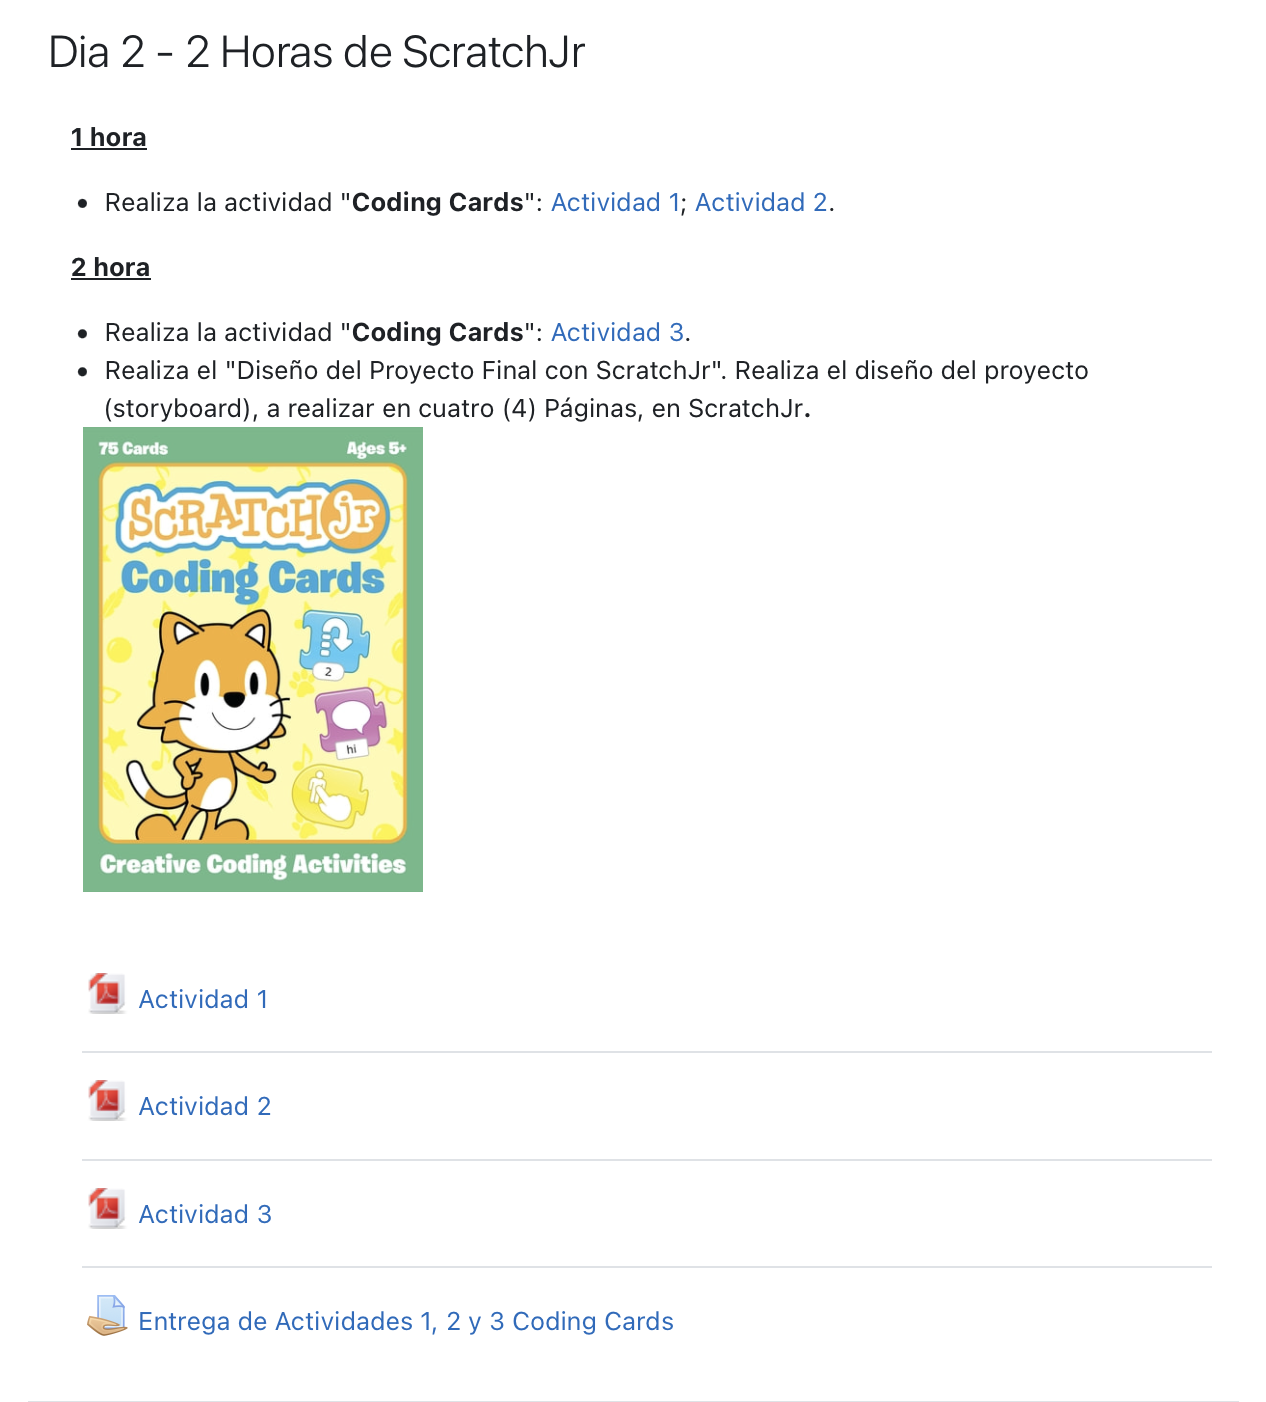
\includegraphics[width=\textwidth]{Fig4.png}
 \end{minipage}%
 \caption{Daily structure of the ScratchJr course.}
 \label{fig3}
 \source{Author’s own elaboration.} 
\end{figure}

\begin{figure}[htbp]
 \centering
 \begin{minipage}{.45\textwidth}
 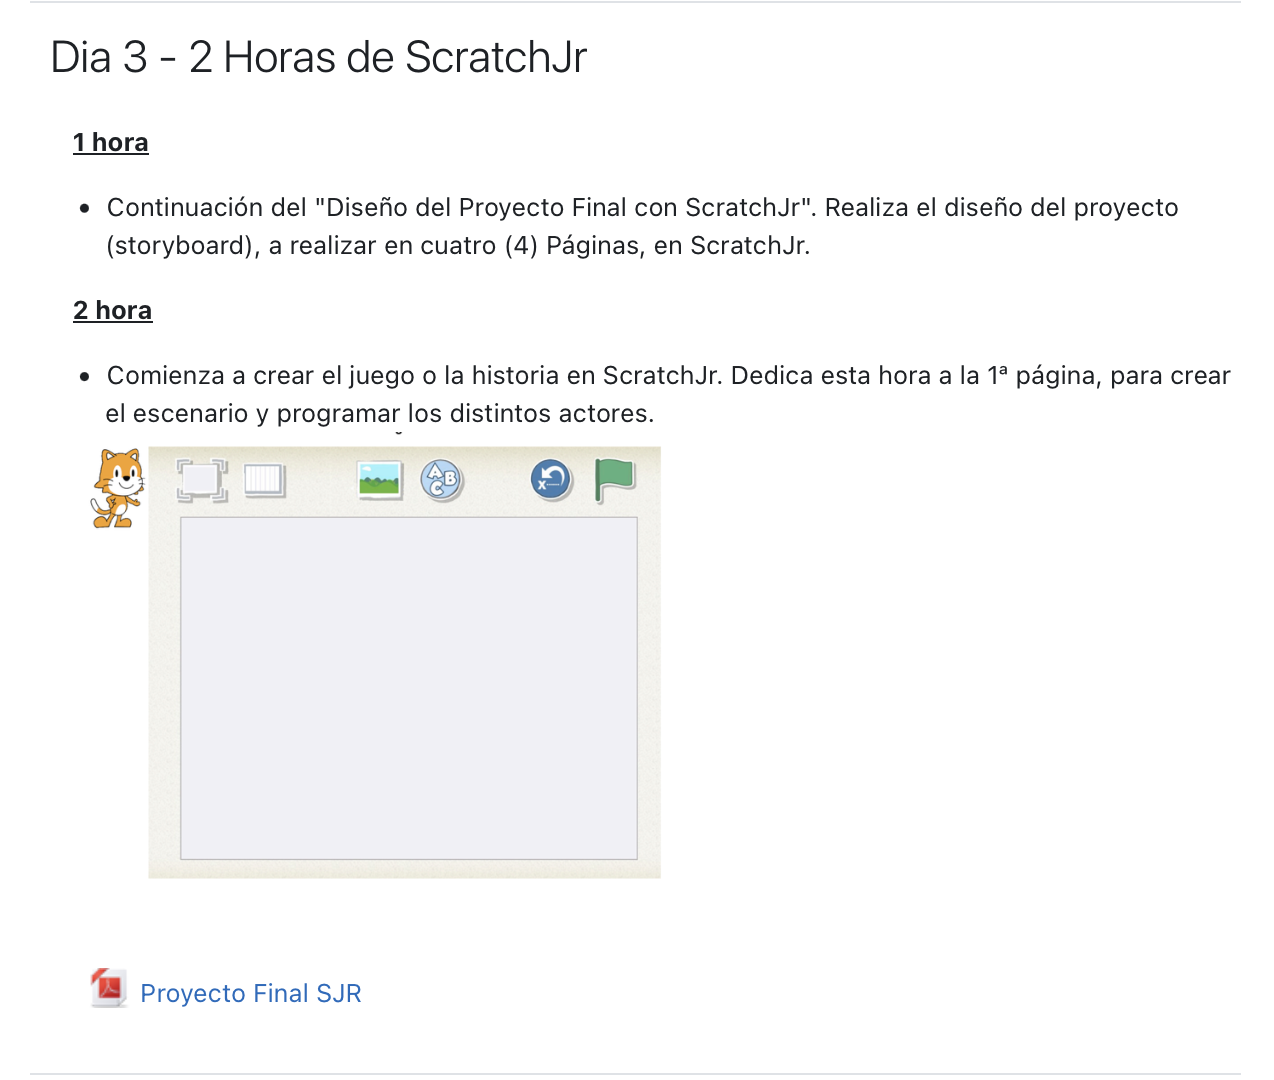
\includegraphics[width=\textwidth]{Fig5.png}
 \end{minipage}%
 \qquad
 \begin{minipage}{0.45\textwidth}
 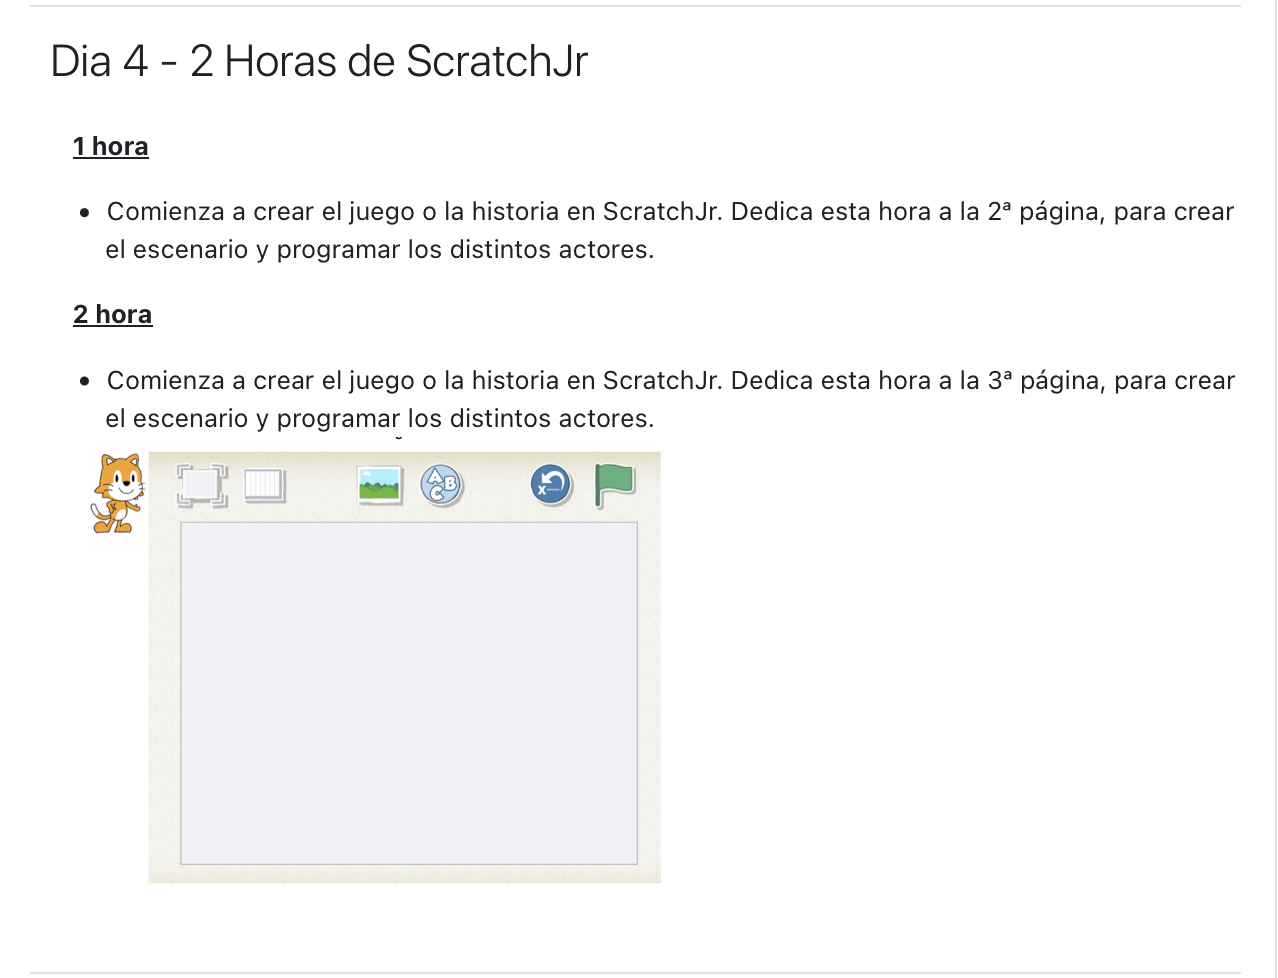
\includegraphics[width=\textwidth]{Fig6.png}
 \end{minipage}%
 \caption{Daily structure of the ScratchJr course.}
 \label{fig4}
 \source{Author’s own elaboration.} 
\end{figure}

\begin{figure}[htbp]
\centering
\begin{minipage}{.8\textwidth}
 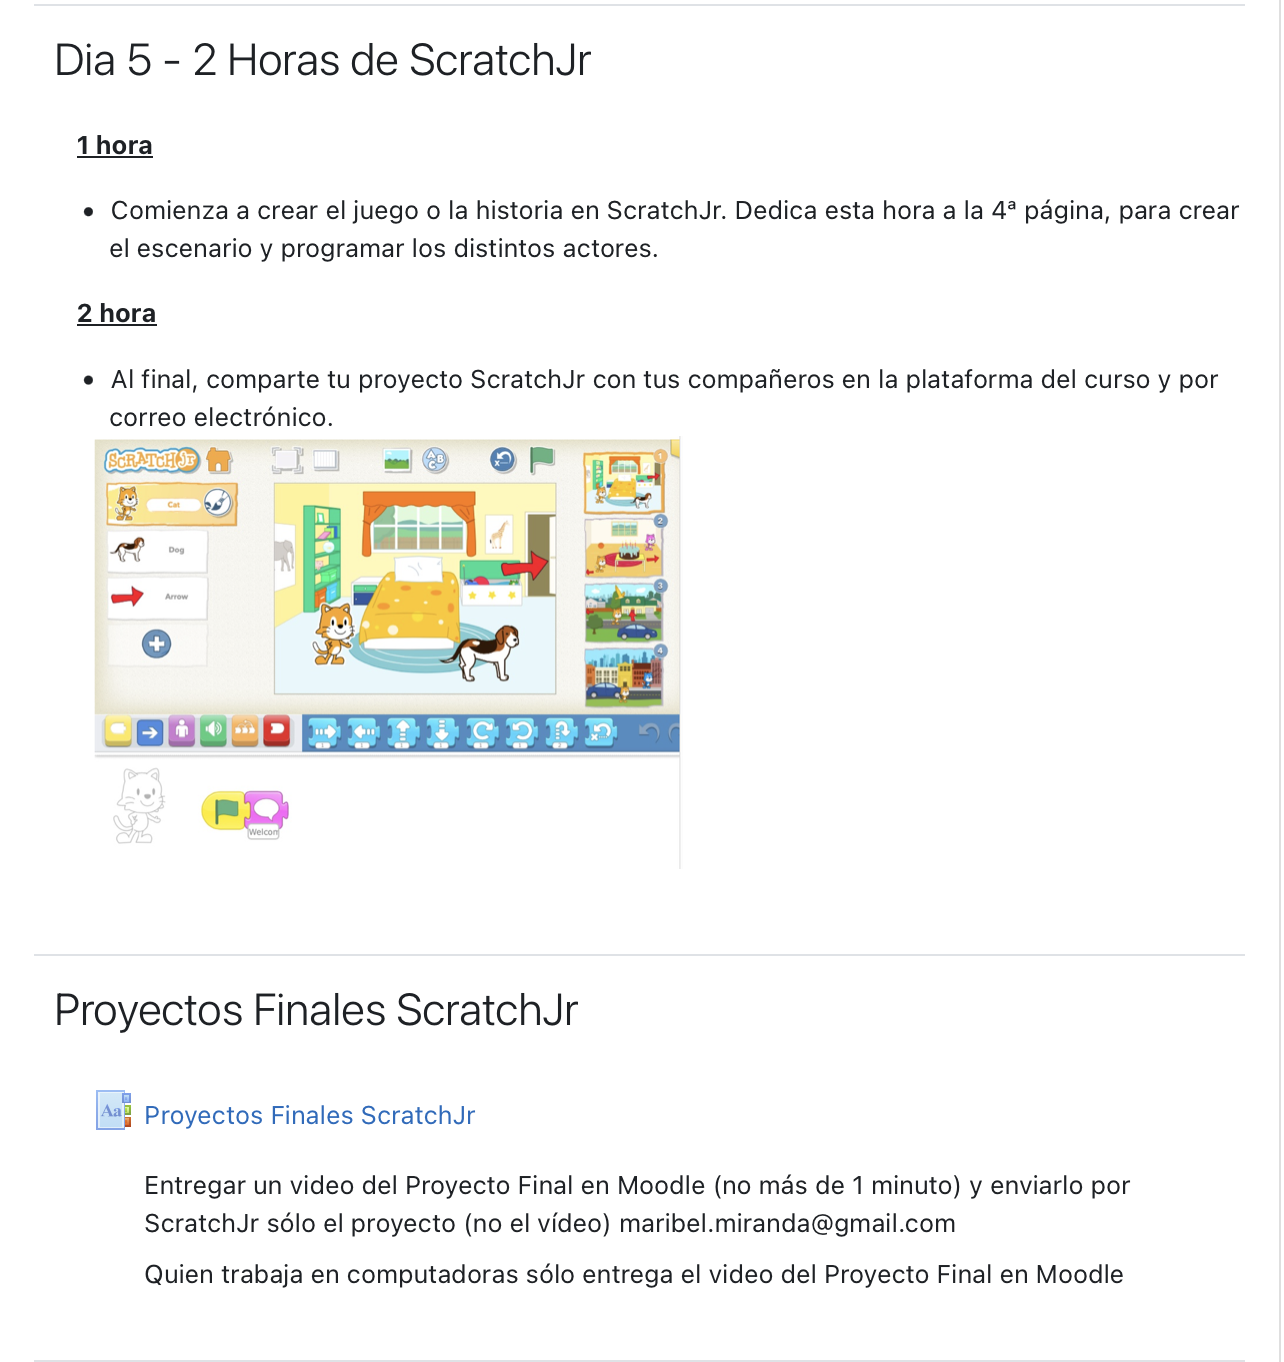
\includegraphics[width=\textwidth]{Fig7.png}
 \caption{Daily structure of the ScratchJr course.}
 \label{fig7}
 \source{Author’s own elaboration.}
\end{minipage}
\end{figure}

\subsection{Implementation}\label{sec-codigos}
The Implementation phase of the ScratchJr course was executed in two distinct stages, facilitating an iterative process of continuous improvement based on participant feedback and evaluation data. These stages comprised: (1) a pilot test to refine the initial design, and (2) the case study, which serves as the focal point of this article.


\subsubsection{Design of the virtual learning environment}\label{sec-contributors-expl}
During the first stage, the ScratchJr course was launched as a pilot program within the Early Childhood Technology Certificate Program at Tufts University (USA) during the 2020/2021 academic year. This initial implementation, conducted in July 2021, targeted a cohort of 25 participants enrolled in the Special Topics: Early Childhood Technology Residency course \cite{mirandapinto2022scratchjr}. The group consisted of education professionals and students specializing in early childhood technology, specifically focusing on the pedagogical application of ScratchJr for young learners.

The objective of this pilot phase was to conduct a comprehensive evaluation of the course, assessing content relevance, instructional clarity, platform navigability, and the efficacy of activities in achieving learning objectives. To this end, participants completed a post-course evaluation questionnaire, providing both qualitative and quantitative data. Key metrics included the clarity of instructional materials, the usability and organization of the Virtual Learning Environment (VLE), overall satisfaction with practical tasks, and the perceived pedagogical utility of the knowledge acquired \cite{mirandapinto2022scratchjr}.

Based on these findings, significant refinements were made to the course design. These improvements included restructuring activities, incorporating supplementary instructional resources, and streamlining the Moodle interface to enhance navigation and module sequencing. These modifications aimed to mitigate identified challenges and enrich the autonomous learning experience, ensuring the course was both accessible and effective for pre-service and in-service teachers.

\subsubsection{Stage 2. Case study}\label{sec-conclusao}
Incorporating the refinements previously outlined, the ScratchJr course was offered to undergraduate students in the Degree in Education at the University of Malaga (Spain), as a specialized component of the curriculum. A total of 48 students enrolled in and completed the course; of these, 28 submitted a final project along with pre- and post-test questionnaires, fulfilling the requirements for the certificate of participation issued by the @rcaComum Association.

Throughout this implementation phase, participants were monitored to evaluate the course's impact on their development of Computational Thinking (CT) and programming competencies. The final project required the creation of an original story or game in ScratchJr, enabling students to apply acquired knowledge within a self-directed creative context. Furthermore, a moderated discussion forum was established on the platform to facilitate experience sharing, peer-to-peer support, and collaborative problem-solving, thereby fostering an active learning community.

To assess the efficacy of the implementation and gather empirical data on learning outcomes, students completed a comprehensive post-test questionnaire featuring both open-ended and closed-ended items. The results (detailed in \textcite{ibanez2023evaluation}) indicated that participants perceived the course as highly valuable and relevant to their future professional careers. Notably, a significant increase was observed in students' self-efficacy regarding the integration of programming tools like ScratchJr into their future educational practices.

\subsection{Evaluation}
Within the ADDIE framework, the Evaluation phase is critical to verifying the quality and overall efficacy of the training program. In this study, a dual evaluation approach was adopted: (1) a formative evaluation, centered on the attainment of learning objectives and the immediate impact on participants' competencies; and (2) a summative course evaluation, designed to identify necessary refinements to the content, delivery, and structural framework for future iterations.

\subsubsection{Formative Assessment}

The formative assessment sought to measure the degree of content mastery and skill acquisition upon course completion, thereby determining the extent to which learning objectives were met. Prior to the intervention, students (n=48) completed a baseline questionnaire regarding general knowledge of Programming Languages in Education. This instrument comprised three sections: (1) introduction; (2) demographic data (gender, age, university, and degree); and (3) specialized knowledge, consisting of seven items five dichotomous, one multiple-choice with an open-entry option, and one qualitative open-ended question.

Subsequently, students engaged with the ScratchJr online course, completing modular assessment activities and submitting a capstone project (as detailed in \Cref{tbl1}). While all 48 students completed the instructional phase, 28 submitted the final project required for certification. Upon completion, these participants (n=28) answered a summative questionnaire consisting of nine items designed to evaluate: (a) mastery of fundamental concepts (programming languages, Computational Thinking, and coding); (b) the perceived impact of the training on their future professional practice; and (c) the competencies acquired for cross-curricular ScratchJr integration.

This final instrument utilized a mix of open-ended, dichotomous, and multi-option Likert-style scales. Results \cite{ibanez2023evaluation} revealed that, prior to the course, students possessed limited foundational knowledge of programming languages (77.1\%), ScratchJr (79.2\%), and Computational Thinking (87.5\%). Notably, 95.8\% were unfamiliar with other child-oriented programming languages, and 97.9\% reported no prior programming proficiency. Following the intervention, participants demonstrated a significant acquisition of coding and CT competencies. Furthermore, between 96.4\% and 100\% of students affirmed the necessity of incorporating CT and ScratchJr into initial teacher education, citing its profound relevance to their prospective professional careers \cite{ibanez2023evaluation}.

\subsubsection{Course evaluation}
Upon completion of the course, students filled out a questionnaire to evaluate the suitability and quality of the course structure, content, and instructional activities \cite{mirandapinto2023evaluation}. This instrument comprised seven items, five of which were dichotomous (yes/no) to assess the relevance, clarity, and adequacy of the provided documents, PDF readings, and learning tasks. Each dichotomous item was paired with an open-ended qualitative field for improvement suggestions, alongside a specific question regarding the overall course framework. Finally, participants provided a global rating of the course using a 5-point Likert scale (where 1 indicates the lowest and 5 the highest level of satisfaction).

The results indicated that 100\% of the students perceived the documentation as well-structured, providing clear information regarding organization, required resources, and activities. Regarding content, 100\% of participants rated the readings as adequate and sufficient for mastering ScratchJr fundamentals. Furthermore, 92.9\% stated that the “Coding Cards” activities were effective for learning core programming concepts, while 96.4\% considered the Storyboard design activity to be a critical preliminary step for the successful execution of the final ScratchJr project. The course achieved an overall satisfaction rating of 4.60 out of 5 \cite{mirandapinto2023evaluation}.

\section{Discussion}
This study has demonstrated the efficacy of the ADDIE instructional model as a robust structural framework for designing and developing a virtual, self-paced course focused on ScratchJr. While other prominent models such as those by \textcite{dick2009systematic,gagne2005principles}, or ASSURE \cite{heinich2002instructional} offer valuable instructional design frameworks, ADDIE distinguishes itself through its practicality and systematic flexibility. This characteristic is particularly advantageous for virtual training environments, as it facilitates the precise alignment of learning objectives, activities, resources, and assessment criteria \cite{hadi2017development}.

The findings reflect a significant enhancement in participants' Computational Thinking (CT) competencies and their proficiency in utilizing ScratchJr as a pedagogical tool. These results align with previous research highlighting the pervasive lack of CT training in Initial Teacher Education (ITE) programs \cite{bers2018scratchjr}, while simultaneously validating the power of well-structured interventions to bridge this gap. The scaffolded integration of resources such as Coding Cards and storyboarding facilitated the progressive mastery of programming concepts. Combined with high participant satisfaction, these outcomes underscore the effectiveness of the adopted pedagogical design.

Furthermore, the course catalyzed a shift in students’ perceptions of educational programming. With approval ratings between 96.4\% and 100\%, participants recognized the necessity of integrating these competencies into their training, signaling a heightened motivation to leverage ScratchJr in their prospective professional practice. This is particularly significant given that educators are the primary agents of innovation and digital literacy from the earliest stages of schooling \cite{bers2014computational}.

Finally, the institutional backing of the Scratch Education Collaborative, alongside its synergy with international projects such as @rcaComum, Kids Media Lab, and KML II (responsible for the MOOC “Programming and Robotics in Primary and Preschool Education” in Portugal), reinforces the sustainability and scalability of this proposal. Such international collaborations facilitate the integration of CT into the curriculum through a multilingual, multicultural, and inclusive lens, resonating with the Coding as Another Language (CAL) curriculum \cite{bers2022coding}.

\section{Conclusion}
The findings of this study support the conclusion that the ADDIE model is a highly effective framework for designing virtual courses centered on educational programming with ScratchJr. Its clear, methodical, and adaptable structure facilitates the strategic planning and execution of training programs that integrate the essential knowledge, skills, and attitudes required for teaching in digital contexts. While other established models such as those by \textcite{dick2009systematic,gagne2005principles}, or ASSURE \cite{heinich2002instructional} provide valuable guidance, ADDIE distinguishes itself through its pragmatic applicability, particularly within technology-mediated instructional environments.

The adopted e-learning modality has proven to be a viable pathway for delivering high-quality, accessible, and flexible training. It effectively addresses geographical and economic barriers, as well as the educational complexities of the post-pandemic era. Beyond fostering critical digital competencies, this proposal has catalyzed a shift in the attitudes of pre-service educators toward the pedagogical use of programming, increasing their self-efficacy in integrating Computational Thinking into their professional practice.

The positive impact of the course evidenced by the measurable growth in foundational knowledge and high participant satisfaction underscores the necessity of embedding programming and CT into both Initial Teacher Education (ITE) and continuing professional development curricula. This experience reinforces the importance of evidence-based instructional design, utilizing scaffolded activities and specialized resources such as Coding Cards and storyboarding.

Furthermore, the international scope of the course, endorsed by the Scratch Education Collaborative (SEC) and integrated into initiatives like the Portuguese MOOC “Programação e Robótica na Educação Básica e Pré-escolar” \cite{amante2023designing}, demonstrates its global relevance and transferability across diverse cultural and educational landscapes.

In conclusion, this proposal stands as a replicable and significant training resource that contributes to narrowing the digital divide and strengthening digital literacy from early childhood. Future research should prioritize longitudinal monitoring of the impact of such training on classroom practice and explore adaptations for various educational levels and sociocultural realities, thereby consolidating the role of teacher education in addressing the challenges of the 21st century.

\printbibliography\label{sec-bib}
% if the text is not in Portuguese, it might be necessary to use the code below instead to print the correct ABNT abbreviations [s.n.], [s.l.]
%\begin{portuguese}
%\printbibliography[title={Bibliography}]
%\end{portuguese}


%full list: conceptualization,datacuration,formalanalysis,funding,investigation,methodology,projadm,resources,software,supervision,validation,visualization,writing,review
\begin{contributors}[sec-contributors]
\authorcontribution{Maribel dos Santos Miranda-Pinto}[conceptualization,methodology,software,validation,formalanalysis,investigation,resources,visualization,projadm,funding,writing,review]
\authorcontribution{Pilar Ibáñez-Cubillas}[conceptualization,methodology,validation,investigation,resources,datacuration,visualization,projadm,writing,review]
\authorcontribution{Slava López-Rodríguez}[validation,resources,writing,review]
\end{contributors}


\begin{dataavailability}
\txtdataavailability{databody} % options: dataavailable, dataonly, databody, datanotav, nodata
\end{dataavailability}

\begin{funding}
Laboratório de Educação a Distância e eLearning (LE@D), financiado por Fundos Nacionais através da FCT, no âmbito dos projetos UID/4372/2025 e UID/PRR/04372/2025. Arcacomum Associação emPortugal: \url{https://www.arcacomum.pt}. Scratch Education Collaborative (SEC): 2022-2024 Cohort.
\end{funding}



\end{document}

